\documentclass[Nike]{tuberlinbeamer}

\usepackage[ngerman]{babel}  % 'babel' muss geladen werden
\usepackage[utf8]{inputenc}  % optional, aber empfehlenswert
\usepackage[square, numbers, comma, sort&compress]{natbib} 
\usepackage[absolute,overlay]{textpos}
\usepackage{multirow}
\usepackage{amsfonts}
\usepackage[load-configurations = abbreviations]{siunitx}

% Die ueblichen Angaben
\title{Veranschaulichung digitaler Steuerprotokolle in der Lichttechnik}
\subtitle{Abschlussvortrag Bachelorarbeit}
\author[Conrad Klaus]{Conrad Klaus}
\institute{Fachgebiet Lichttechnik}

\newcommand{\customcite}[1]{
	\vskip0pt plus 1filll
	\color{grau}
	\raggedleft \tiny Bilder: \cite{#1}
}

\begin{document}

\begin{frame}
	\maketitle
\end{frame}
\begin{frame}{Agenda}
	\tableofcontents
\end{frame}


\section{Thema der Bachelorarbeit}


\begin{frame}{Thema}
	\begin{tabular}{cl}  
		\parbox{0.45\linewidth}{
			\begin{itemize}
				\item Vergleich aktuell verwendeter Lichtsteuerprotokolle
				\item Projekt: Anschauliche Erklärung des DMX Protokolls
				\item DMX Platine
				\item Decodierung: DMX Signal
				\item DMX Protokoll Visualisierung
				\item Gehäuse
			\end{itemize}
		}
		&
		\begin{tabular}{c}
			\includegraphics[height=\textheight - 13pt]{pictures/Problemstellung}
		\end{tabular}
	\end{tabular}
	\customcite{problemstellung}
\end{frame}

\section{Steuerprotokolle}

\begin{frame}{DALI - Digital Addressable Lighting Interface}
	\centering
	\begin{itemize}
		\item Gebäudebeleuchtung
		\item 64 Adressen, 16 Gruppen, 8 Bit Wertebereich
		\item Strom- und Datenkabel kombinierbar
	\end{itemize}

   	\begin{tabular}{cl}  
		\begin{tabular}{c}
				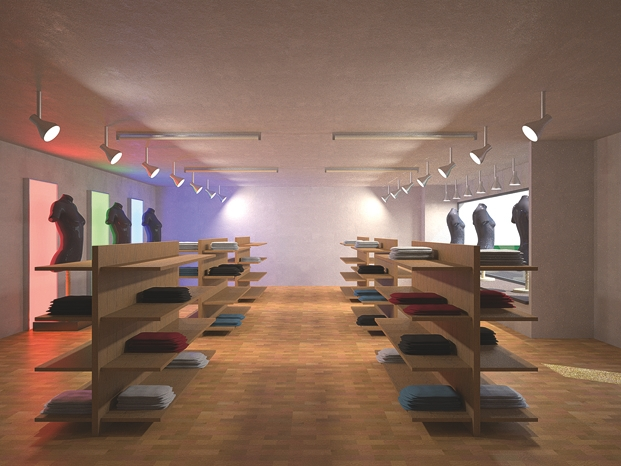
\includegraphics[width=\textwidth/2 - 25pt]{pictures/DaliSchauraumTag}\\
				Lichtszene bei Tag
		\end{tabular}
		& 
	\begin{tabular}{c}
		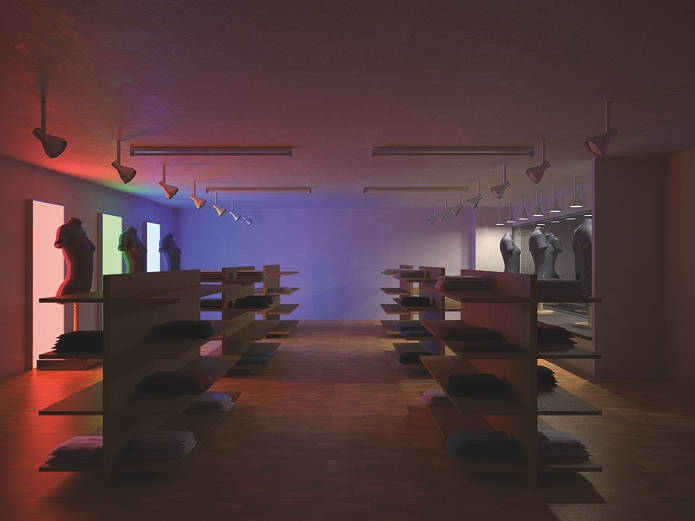
\includegraphics[width=\textwidth/2 - 25pt]{pictures/DaliSchauraumNacht}\\
		Lichtszene bei Nacht
	\end{tabular}
	\end{tabular}

	\customcite{dmx_demo, dmx_cable}
\end{frame}


\begin{frame}{DALI - Digital Addressable Lighting Interface}
	\centering
	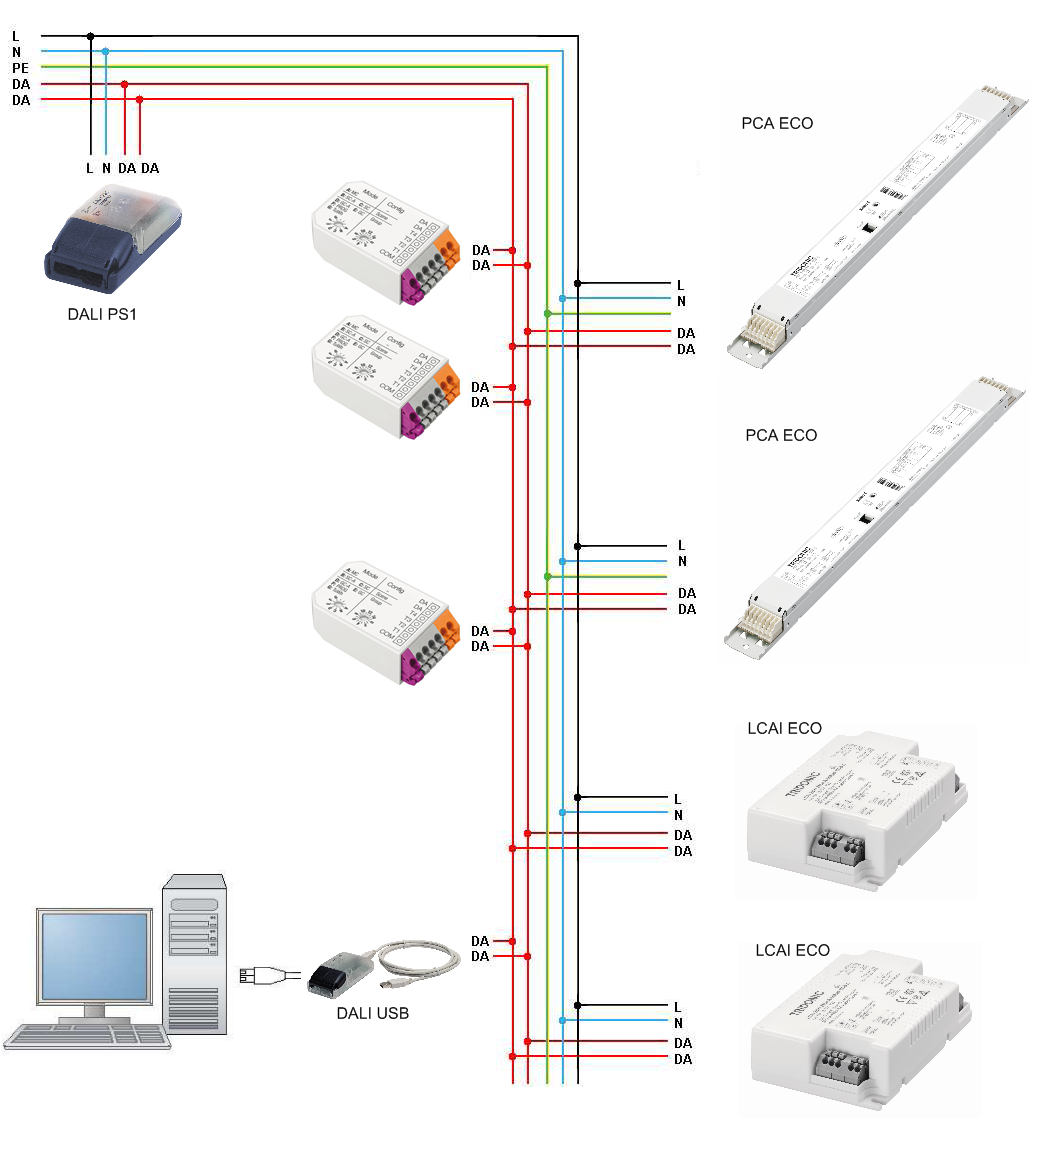
\includegraphics[width=\textwidth/2 - 25pt]{pictures/DaliInstallation.png}\\
	DALI Verkabelungsdiagramm
	\customcite{rpi}
\end{frame}

\begin{frame}{DMX - Digital Multiplex}
	\begin{tabular}{cl}  
		\begin{tabular}{c}
			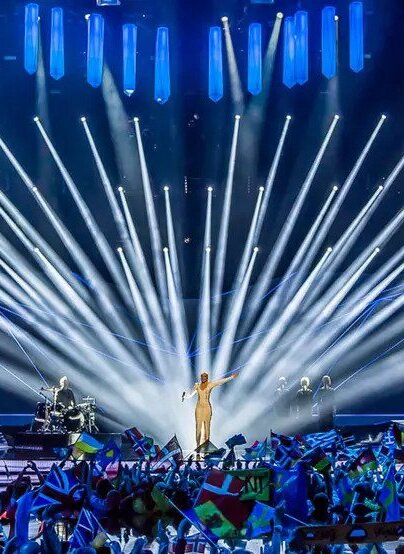
\includegraphics[height=\textheight - 13pt]{pictures/dmx-demo}
		\end{tabular}
		& \parbox{0.5\linewidth}{
			\emph{DMX Protokoll}
			\begin{itemize}
				\item Digital Multiplex (DMX) steuert Leuchten
				\item Farbe, Helligkeit, Ausrichtung etc.
				\item 512 Kanäle mit Wertebereich 0-255
			\end{itemize}
			\vspace{3ex}
			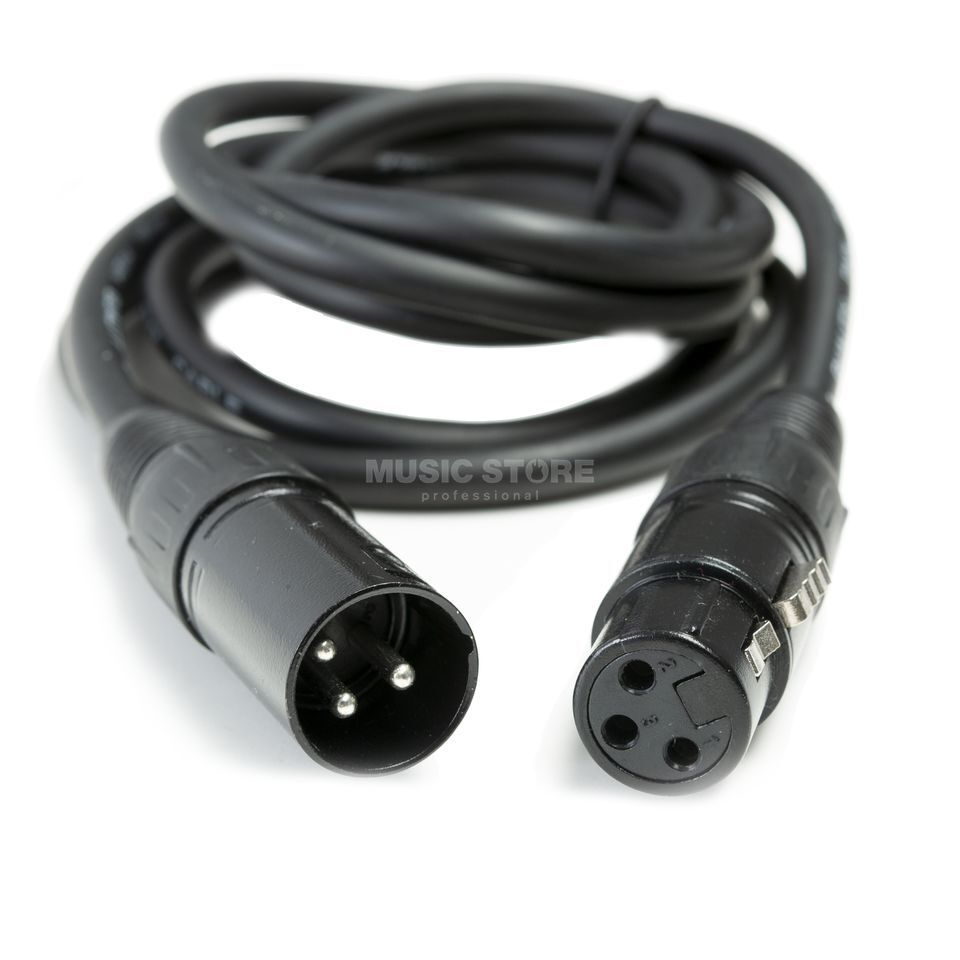
\includegraphics[scale= 0.1]{pictures/dmx-cable}
		}
	\end{tabular}
	\customcite{led_matrix_lightshow, dmx_cable}
\end{frame}


\begin{frame}{DMX - Digital Multiplex}
	\centering
	\begin{itemize}
		\item Reihenschaltung
		\item Ende des Busses sollte terminiert werden
		\item Zentrale Steuerung
	\end{itemize}
	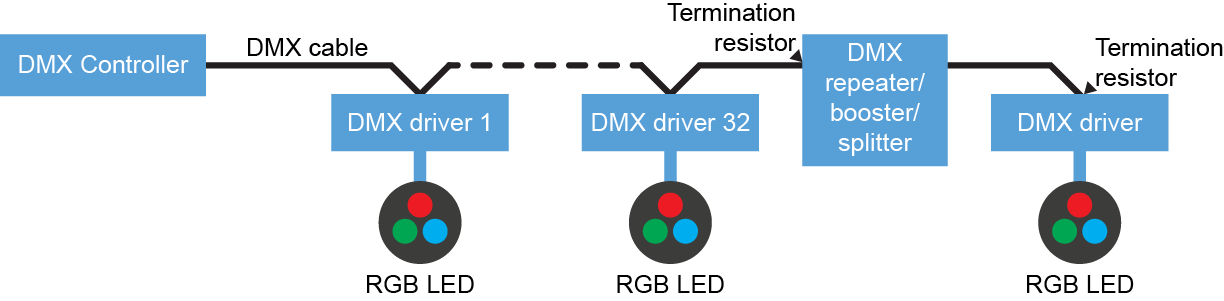
\includegraphics[width=\textwidth - 25pt]{pictures/dmxWiringDiagram.png}\\
	DMX Verkabelungsdiagramm
	\customcite{dmx_timing}
\end{frame}


\begin{frame}{ZigBee}
	\centering
	\begin{tabular}{cl}  
		\begin{tabular}{c}
			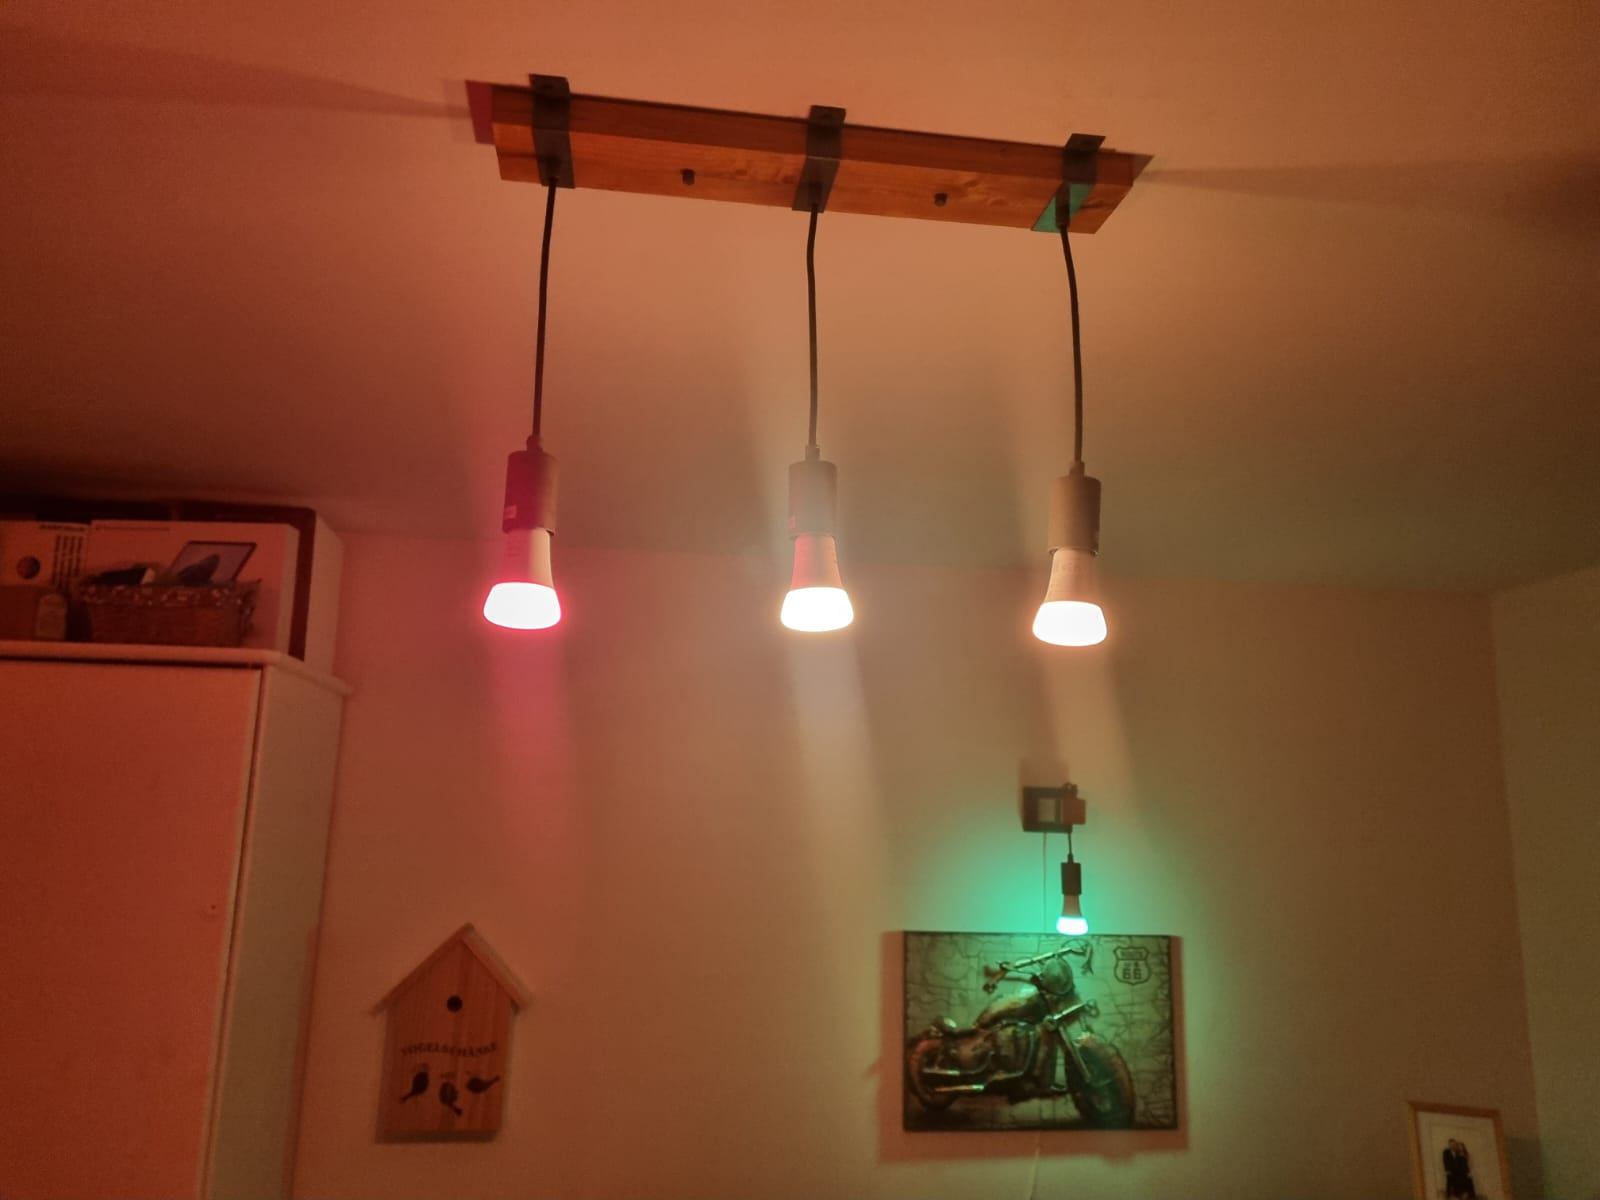
\includegraphics[scale= 0.09]{pictures/phillipsUseCase.jpeg}\\
			Exemplarische Anwendung im Smarthome
		\end{tabular}
		& \parbox{0.5\linewidth}{
			\begin{itemize}
				\item Entwickelt für Smart Home Anwendungen
				\item Kabelose Übertragung
				\item Einfache Nachrüstung
			\end{itemize}
		}
	\end{tabular}
\end{frame}


\begin{frame}{MIDI - Musical Instrument Digital Interface}
	\centering
	\begin{tabular}{cl}  
		\begin{tabular}{c}
			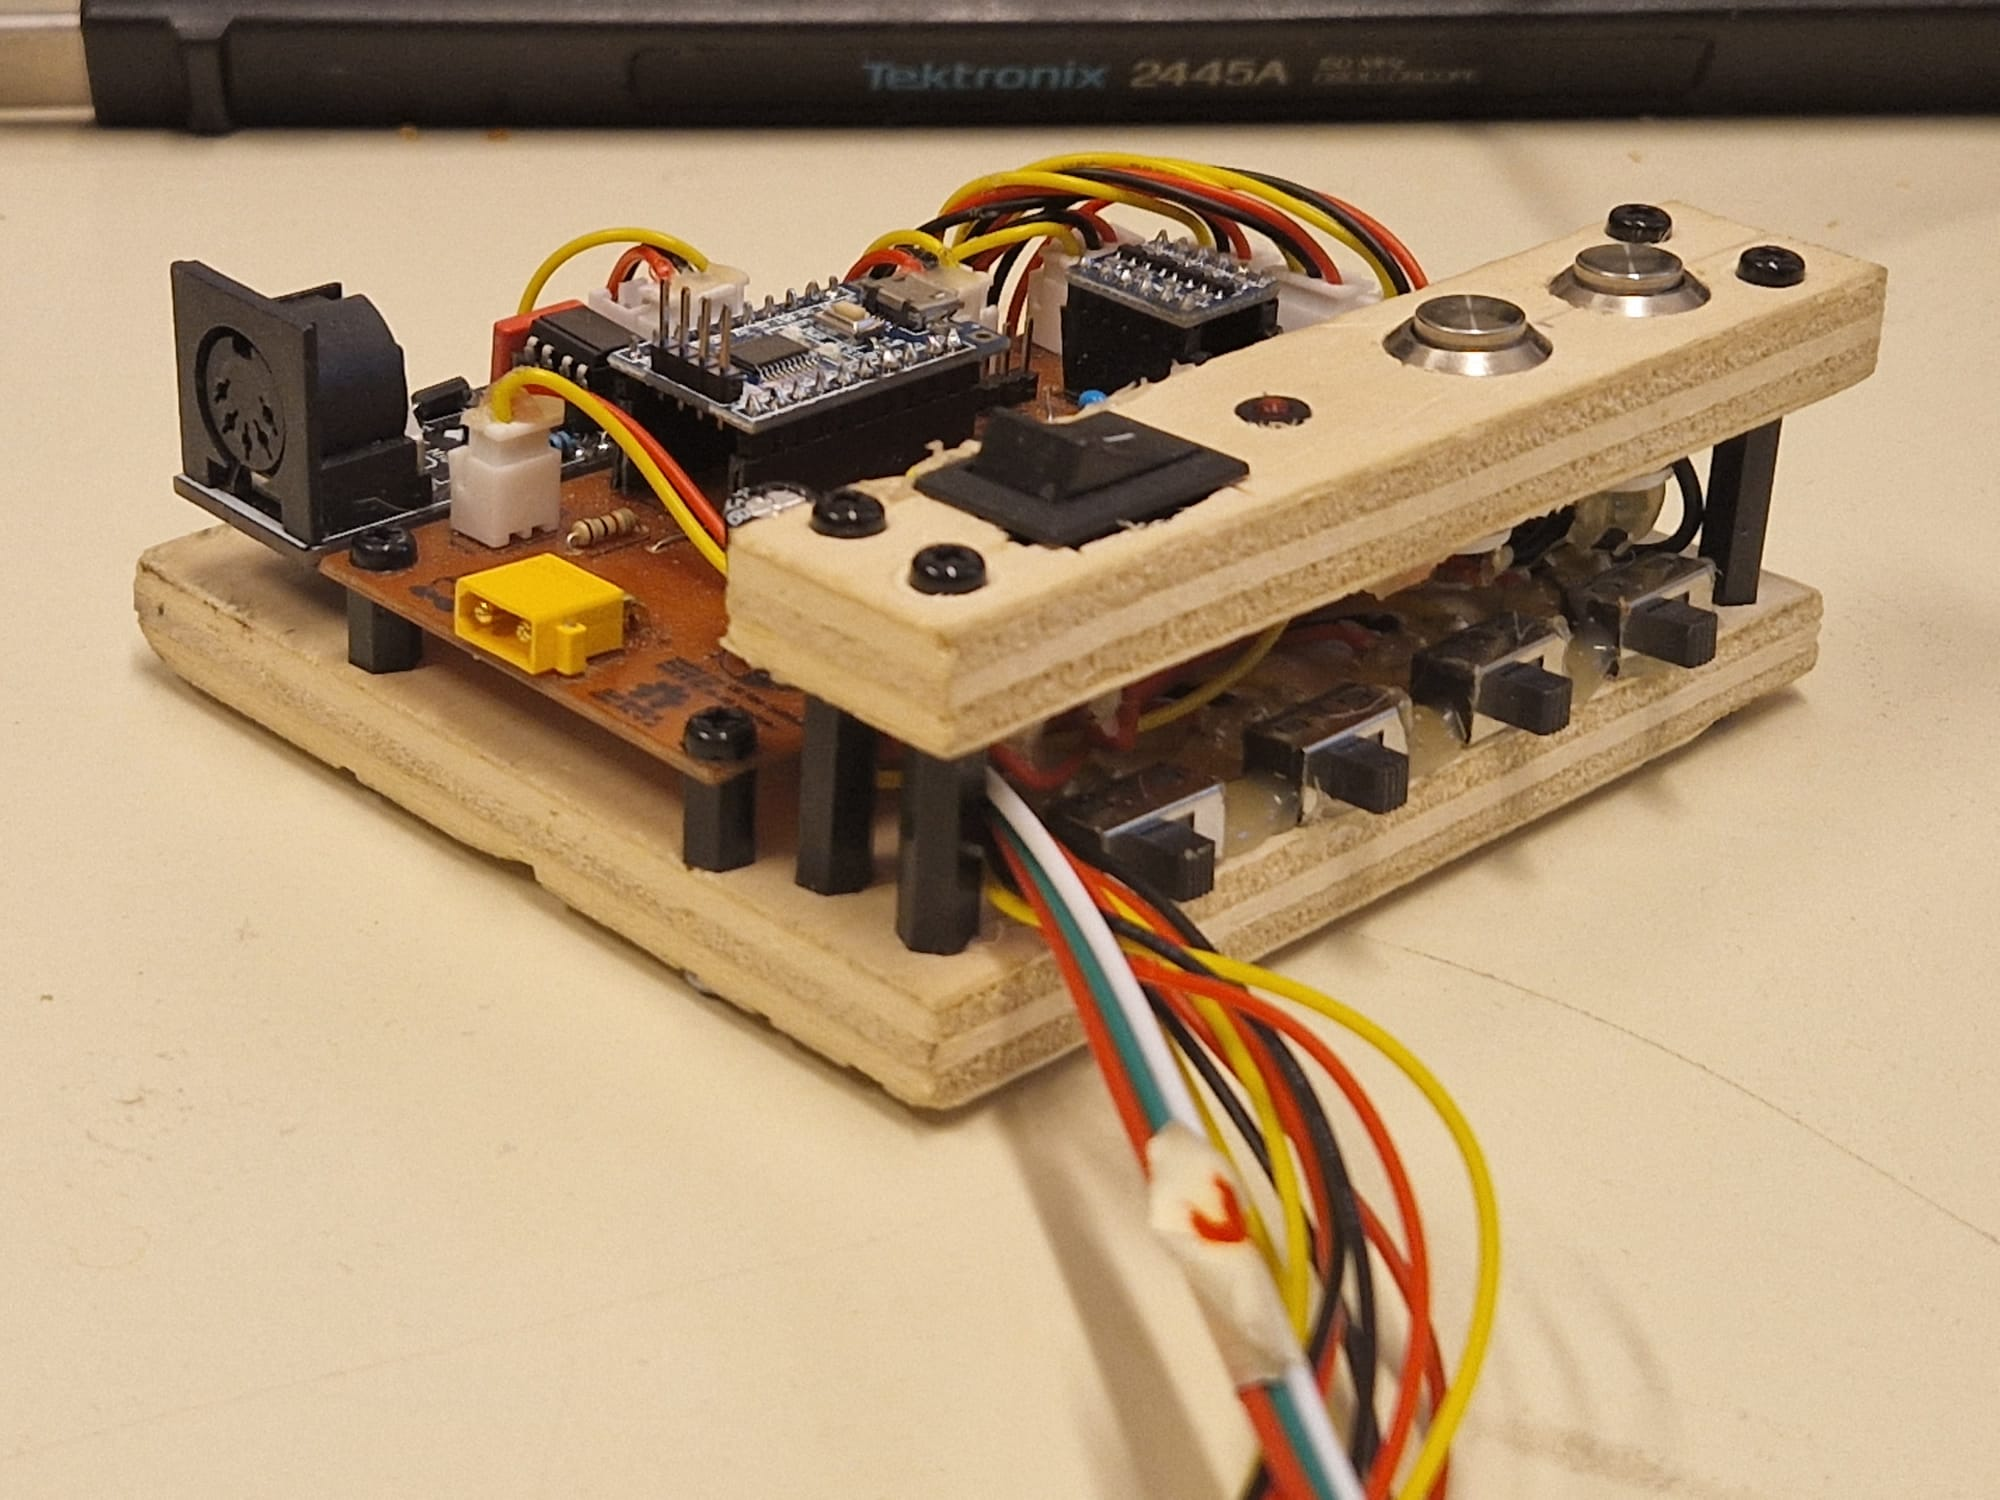
\includegraphics[scale= 0.07]{pictures/midiUseCase.jpeg}\\
			MIDI Lichtsteuergerät aus der Hobbyszene
		\end{tabular}
		& \parbox{0.5\linewidth}{
			\begin{itemize}
				\item Entwickelt für Musik
				\item Ton-An/ Ton-Aus Signale, mit Parametern
				\item Übertragung: Event basiert
			\end{itemize}		
		}
	\end{tabular}
	\customcite{led_matrix_lightshow}
\end{frame}


\begin{frame}{Übersicht der Protokolle}
\begin{table}
	\centering
	\resizebox{\textwidth}{!}{ %
		\begin{tabular}{ |c|c|c|c|c| } 
			\hline
			Kategorie / Protokoll & DALI & DMX & MIDI & ZigBee \\
			\hline
			Aktualisierungsrate & 30 Hz & 44 Hz & Signal basiert & Netzwerk abhängig \\
			Datenrate in $\frac{\SI{}{\kilo\bit}}{\SI{}{\s}}$ & 1,2  & 250 & 31.25 & 40 - 250 \\
			Unterschiedliche Kanäle & 64 Adressen & 512 Kanäle & 16 Geräte &  65,534 Geräte\\
			Topologie & Bus & Bus & Bus & Mesh (Peer-To-Peer) \\
			Exemplarische Verwendung & Häuser & Bühnen & Hobby-/ Musikszene & Intelligentes Zuhause \\
			\hline
	\end{tabular}}
	\caption{Lichtsteuer Protokolle im Vergleich}
	\label{tab:LightProtokollComparison}
\end{table}
\end{frame}



\section{Hardware}

\begin{frame}{Hardware - LED Matrix}
	\begin{tabular}{cl}  
		\begin{tabular}{c}
			
\includegraphics[width=\textwidth / 2 - 30pt]{pictures/LedMatrix}\\
			LED Matrix
		\end{tabular}
		& 
		\begin{tabular}{c}
		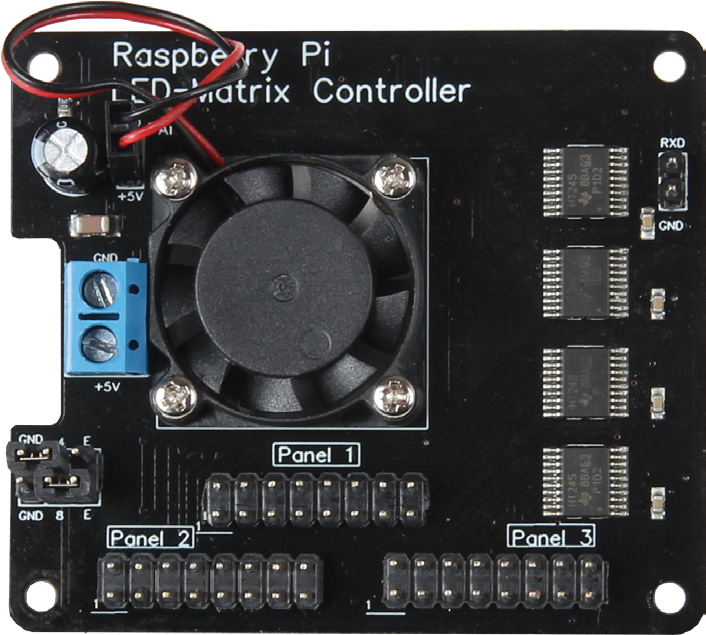
\includegraphics[width=\textwidth/2 - 30pt]{pictures/LedMatrixControllerPlatine}\\
		Steuerplatine: LED Matrix
	\end{tabular}
	\end{tabular}
	\customcite{led-matrix-example, led-matrix-example}
\end{frame}


\begin{frame}{Gehäuse}
	\begin{tabular}{cl}  
		\begin{tabular}{c}
			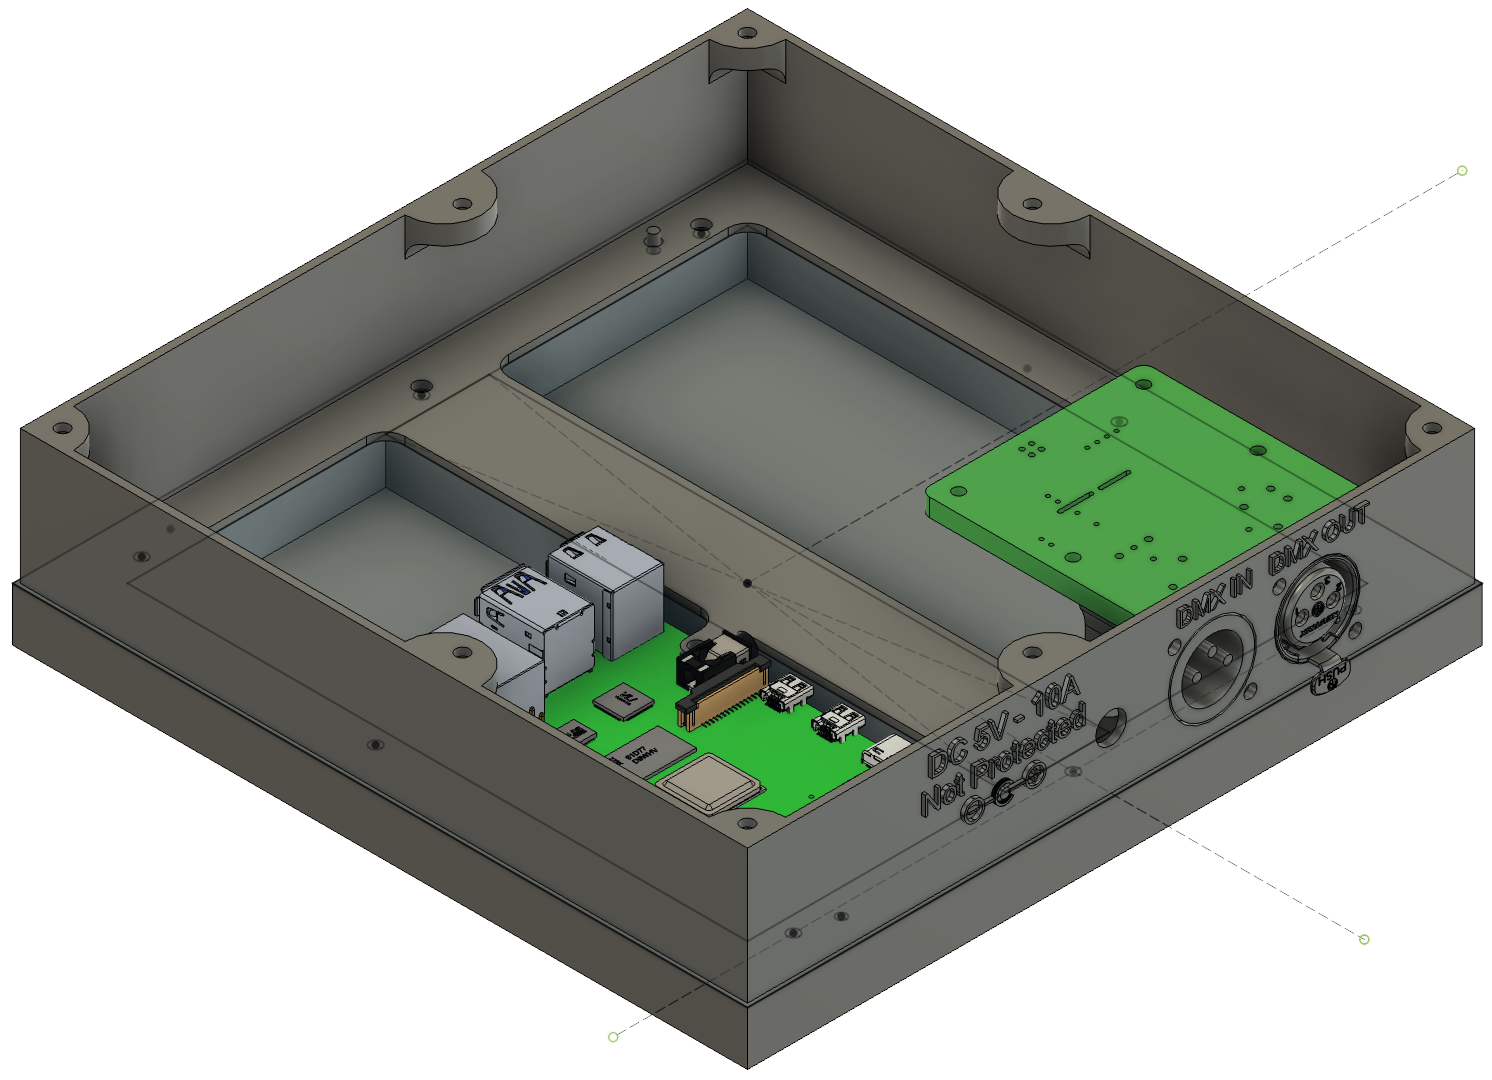
\includegraphics[width=\textwidth/2 - 30pt]{pictures/DmxCaseSideways}\\
			Seitenansicht
		\end{tabular}
		& 
		\begin{tabular}{c}
			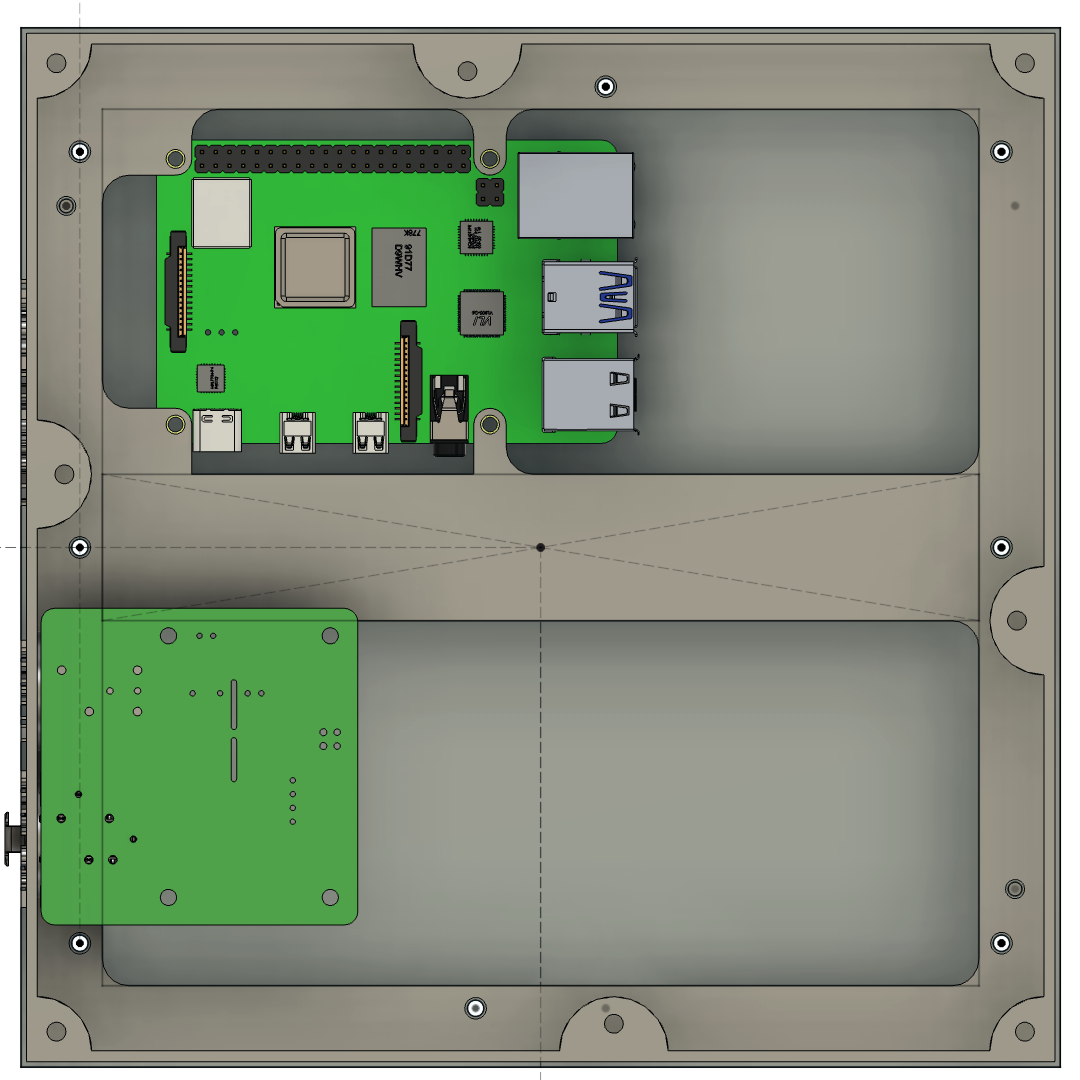
\includegraphics[width=\textwidth/2 - 30pt]{pictures/DmxCaseTop}\\
			Topansicht
		\end{tabular}
	\end{tabular}
\end{frame}

\begin{frame}{Platine}
		\centering
	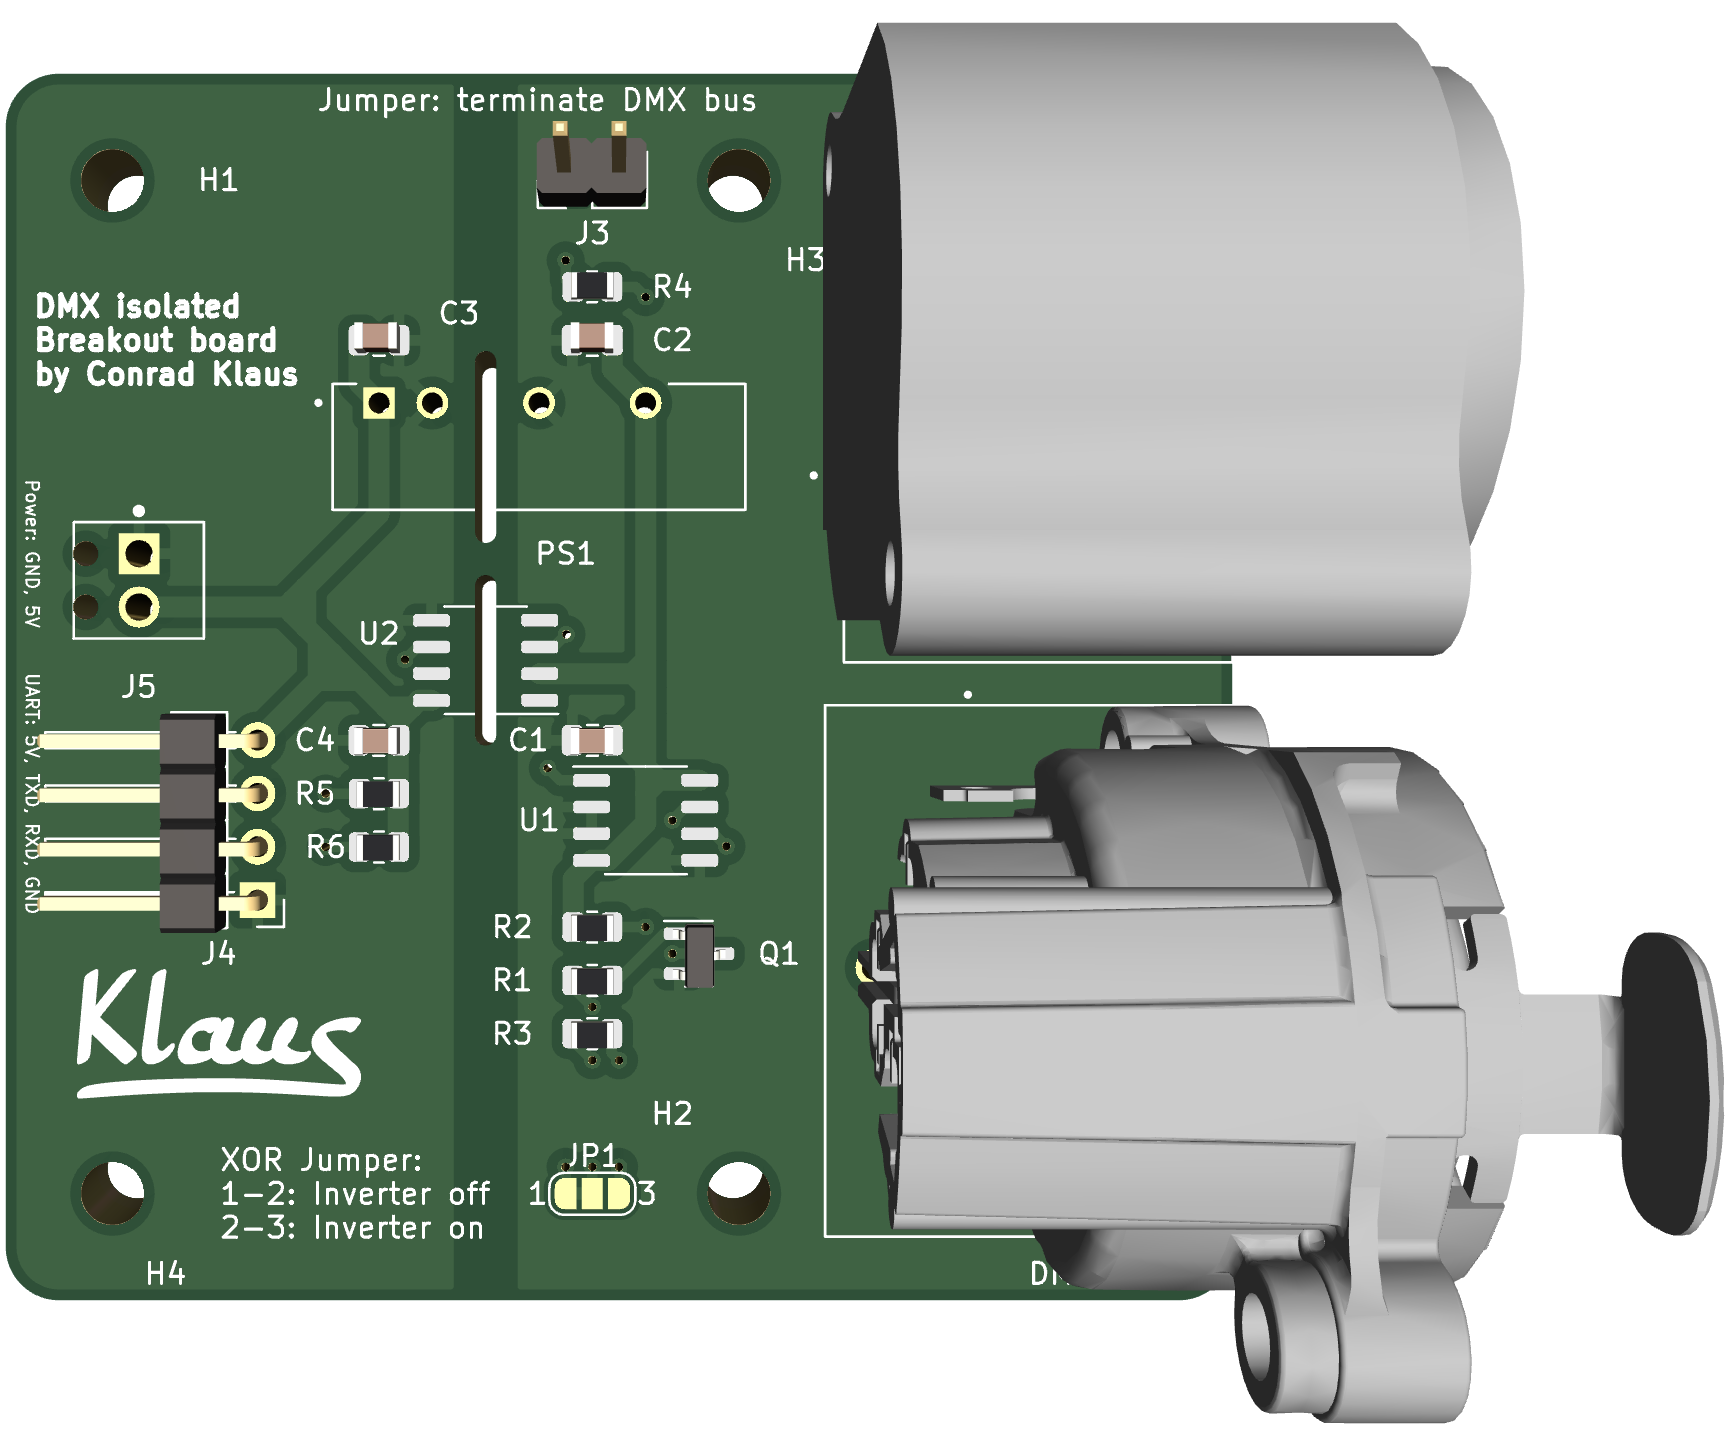
\includegraphics[height=\textheight - 25pt]{pictures/pcbDmxBreakout3dView.png}\\
	Elektronisch Isolierter DMX Eingang
\end{frame}

\begin{frame}{Logik Analysator}
	\centering
	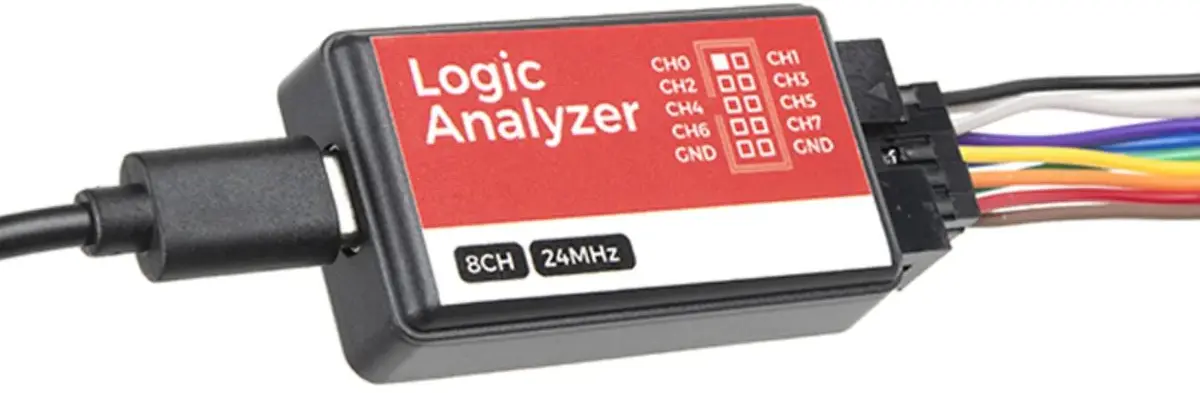
\includegraphics[width=\textwidth - 25pt]{pictures/usb-logic-analyzer-side}\\
	Logik Analysator
	\customcite{fragen}
\end{frame}

\section{Technische Details DMX}
\begin{frame}{Technische Details DMX}
	\centering
	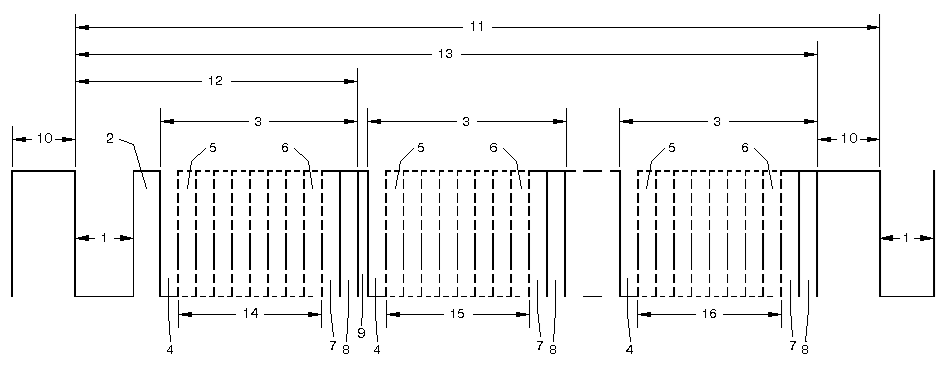
\includegraphics[width= \textwidth - 20pt]{pictures/DmxTimingFrame.png}
	\resizebox{\textwidth}{!}{ %
		\begin{minipage}{0.5 \linewidth}
			\centering
			\tiny{
				\begin{tabular}{ r l}
					1: 	& Space for Break\\
					2:	& Mark after Break (MAB)\\
					3:	& Slot Time\\
					4:	& START Bit\\
					5:	& Least Significant Data Bit\\
					6:	& Most Significant Data Bit\\
					7, 8:	& Stop Bit\\
					9:	& Mark Time between slots\\
					
				\end{tabular}
			}
		\end{minipage}\hfill
		\begin{minipage}{0.5 \linewidth}
			\tiny{
				\begin{tabular}{ r l}
					10:	& Mark before break (MBB)\\
					11:	& Break to break Time\\
					12:	& Reset Sequence (Break, MAB, Start
					Code)\\
					13:	& DMX512 Packet\\
					14:	& Start code (Slot 0 Data)\\
					15:	& Slot 1 Data\\
					16:	& Slot nnn Data (Maximum 512)\\
				\end{tabular}
			}
		\end{minipage}
	}
\customcite{dmx_timing}
\end{frame}


\begin{frame}{Technische Details DMX}
	\centering
	\begin{table}[H]
		\centering
		\resizebox{\textwidth}{!}{ %
			\begin{tabular}{ |c|c|c|c|c|c| } 
				\hline
				Nr. & Beschreibung & Min & Typ & Max & Einheit \\
				\hline
				-  & Bit Übertragungsrate	&	245 	& 250 	& 255 	& $\frac{\SI{}{\kilo\bit}}{\SI{}{\s}}$ \\
				-  & Bitlänge	&	3.92	&  4	& 4.08 	& µs\\
				-  & minimale Aktualisierungszeit bei 513 Bytes 	& – & 22.7	& – & ms\\
				-  & maximale Aktualisierungsrate bei 513 Bytes & – & 44	& – & $\frac{\SI{}{Aktualisierungen}}{\SI{}{\s}}$\\
				1  & Raum für Pause 	& 92 & 176 & – &  µs\\
				2  & Mark Break (MAB)		& 12 $|$  – & – & – $|$  $<$ 1.00 & µs $|$  s \\
				9  & Markierungszeit zwischen Bytes 	& 0  & – & $<$ 1.00 & s\\
				10 & Mark Before BREAK (MBB)	& 0  & – & $<$ 1.00 & s\\
				11 & Pause zu Pause Zeit & 1204 $|$ – & – & – $|$ 1.00   & µs $|$ s \\
				13 & DMX512 Paket & 1204 $|$ – & – & – $|$ 1.00 & µs $|$ s \\
				\hline
		\end{tabular}}
		\caption{Zeitdiagramm}
		\label{tab:timingChart}
	\end{table}
\end{frame}

\section{Software}
\begin{frame}{Bildschirmausgabe}
	\centering
	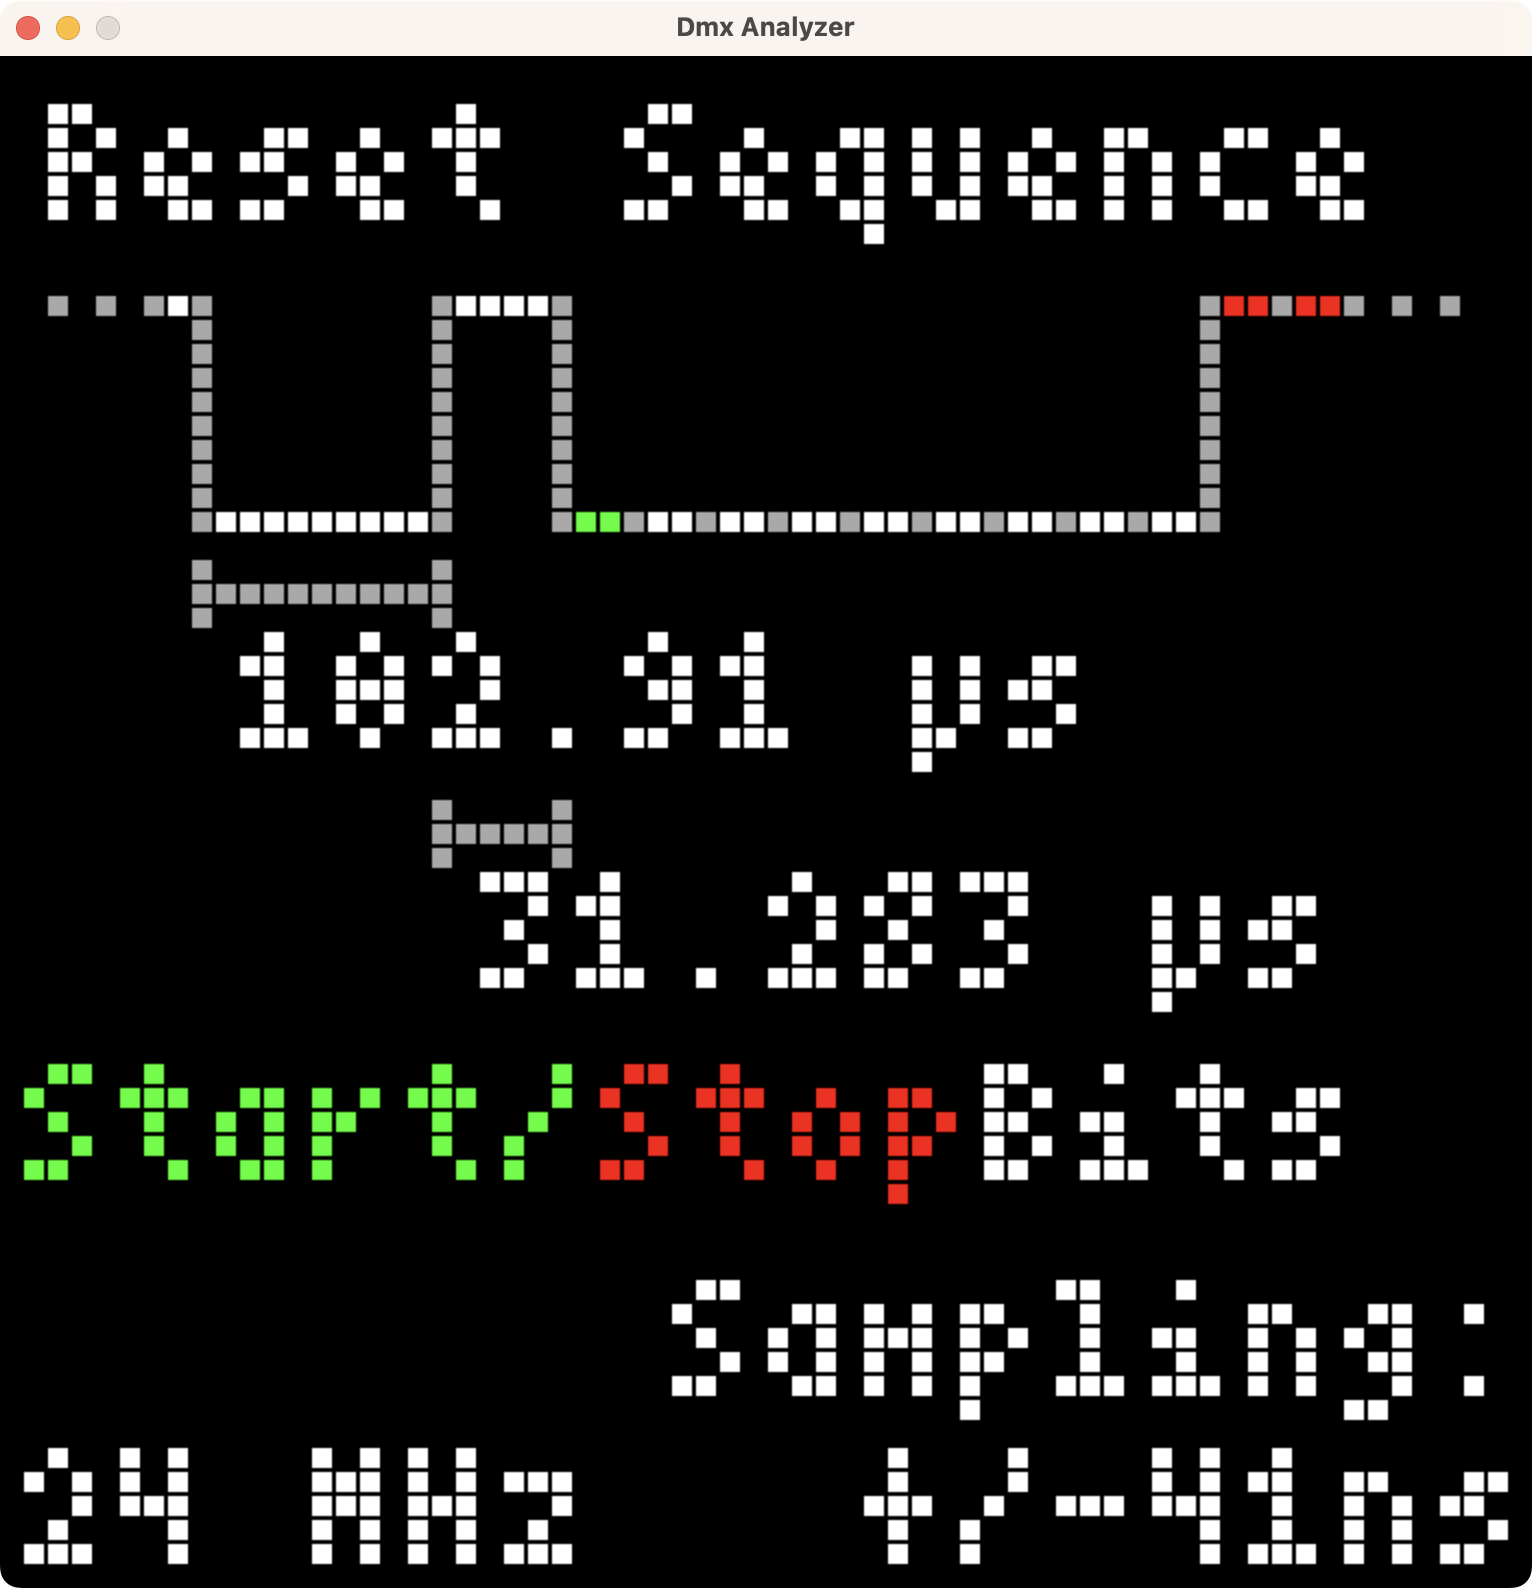
\includegraphics[height=\textheight - 25pt]{pictures/screenshotResetSequence}\\
	Reset Sequenz
	
\end{frame}

\begin{frame}{Bildschirmausgabe}
	\centering
	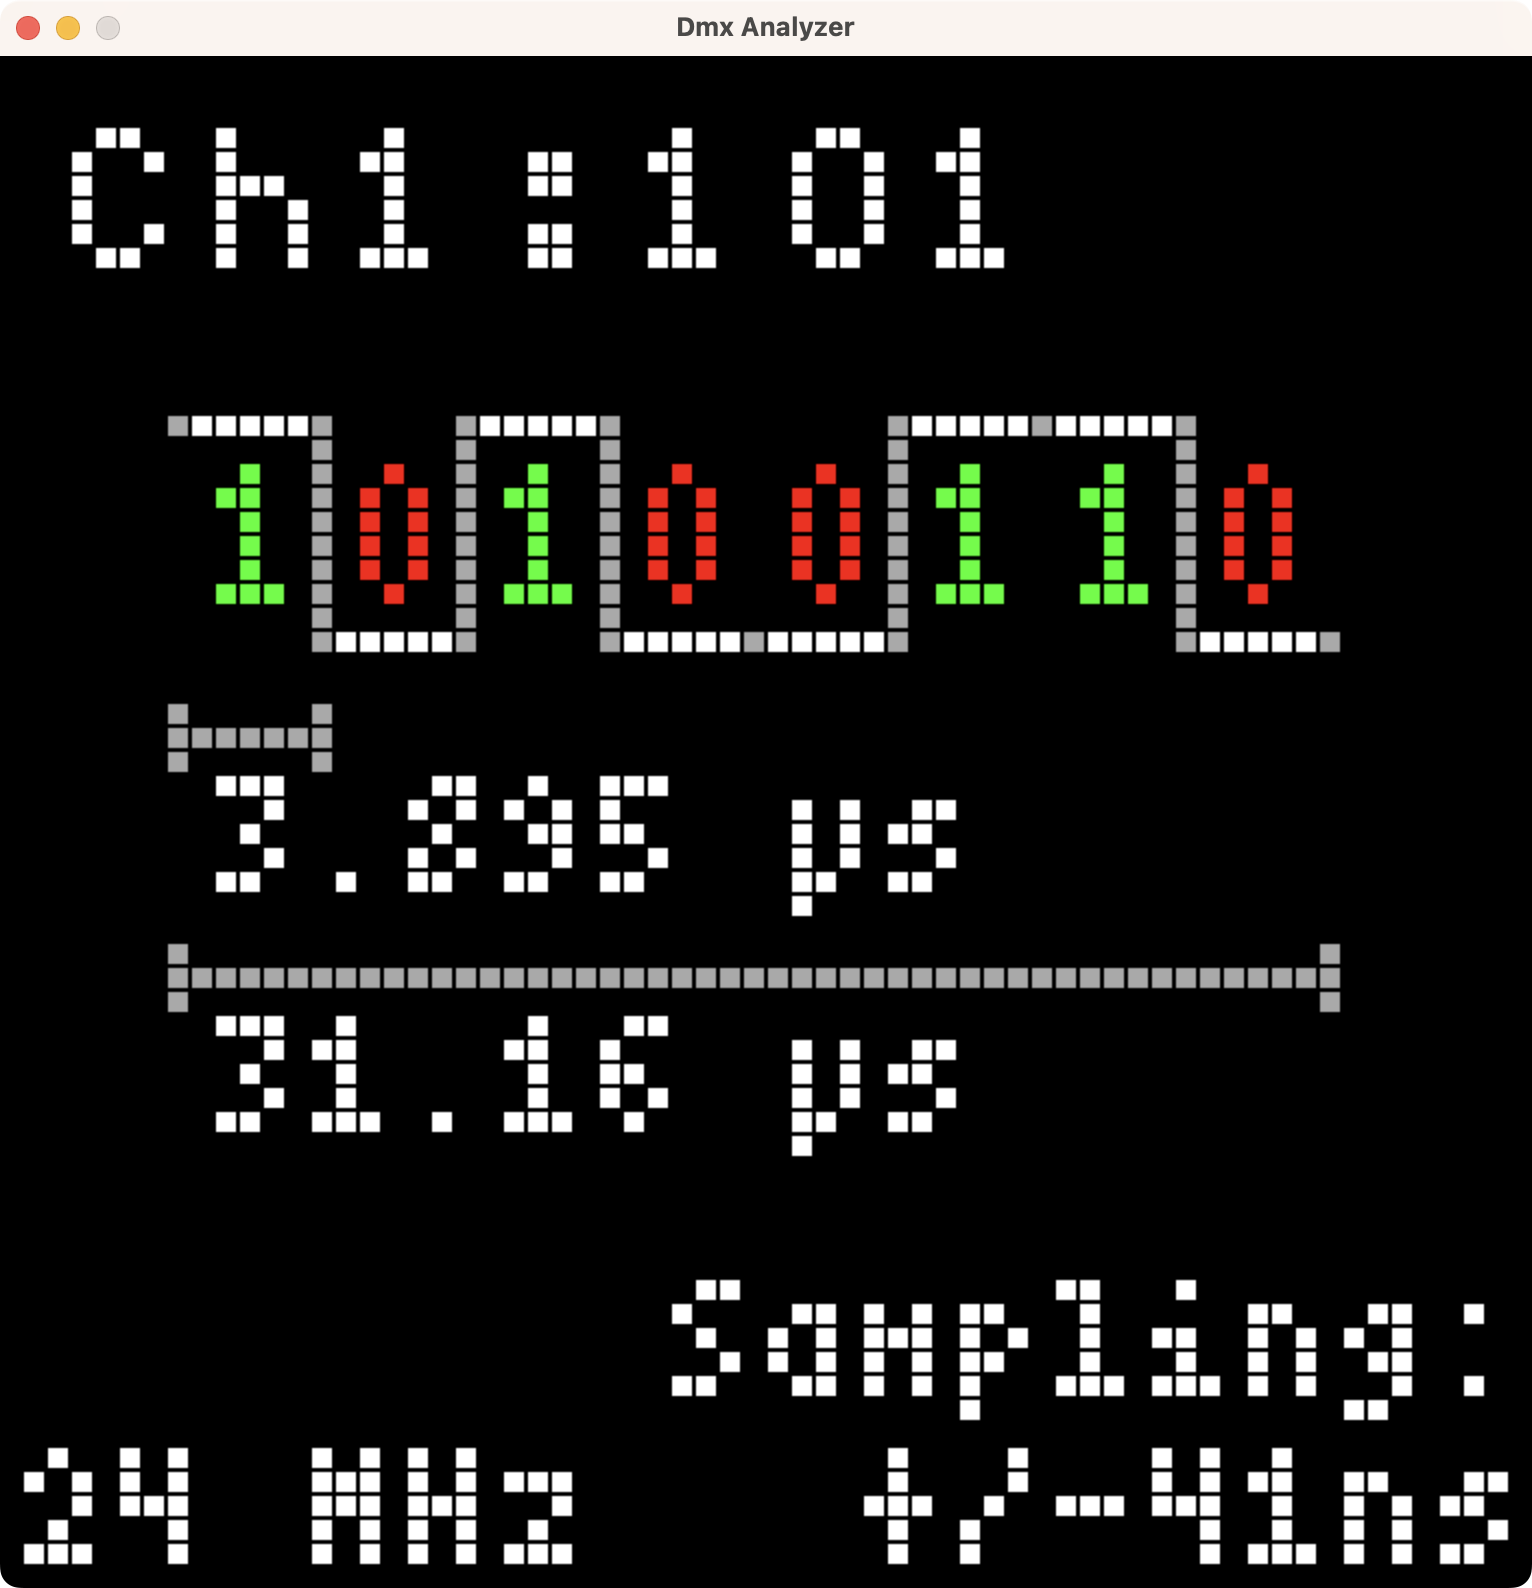
\includegraphics[height=\textheight - 25pt]{pictures/screnshotChannel1}\\
	Kanal 1
\end{frame}


\begin{frame}{Bildschirmausgabe}
	\centering
	\begin{tabular}{cl}  
		\begin{tabular}{c}
			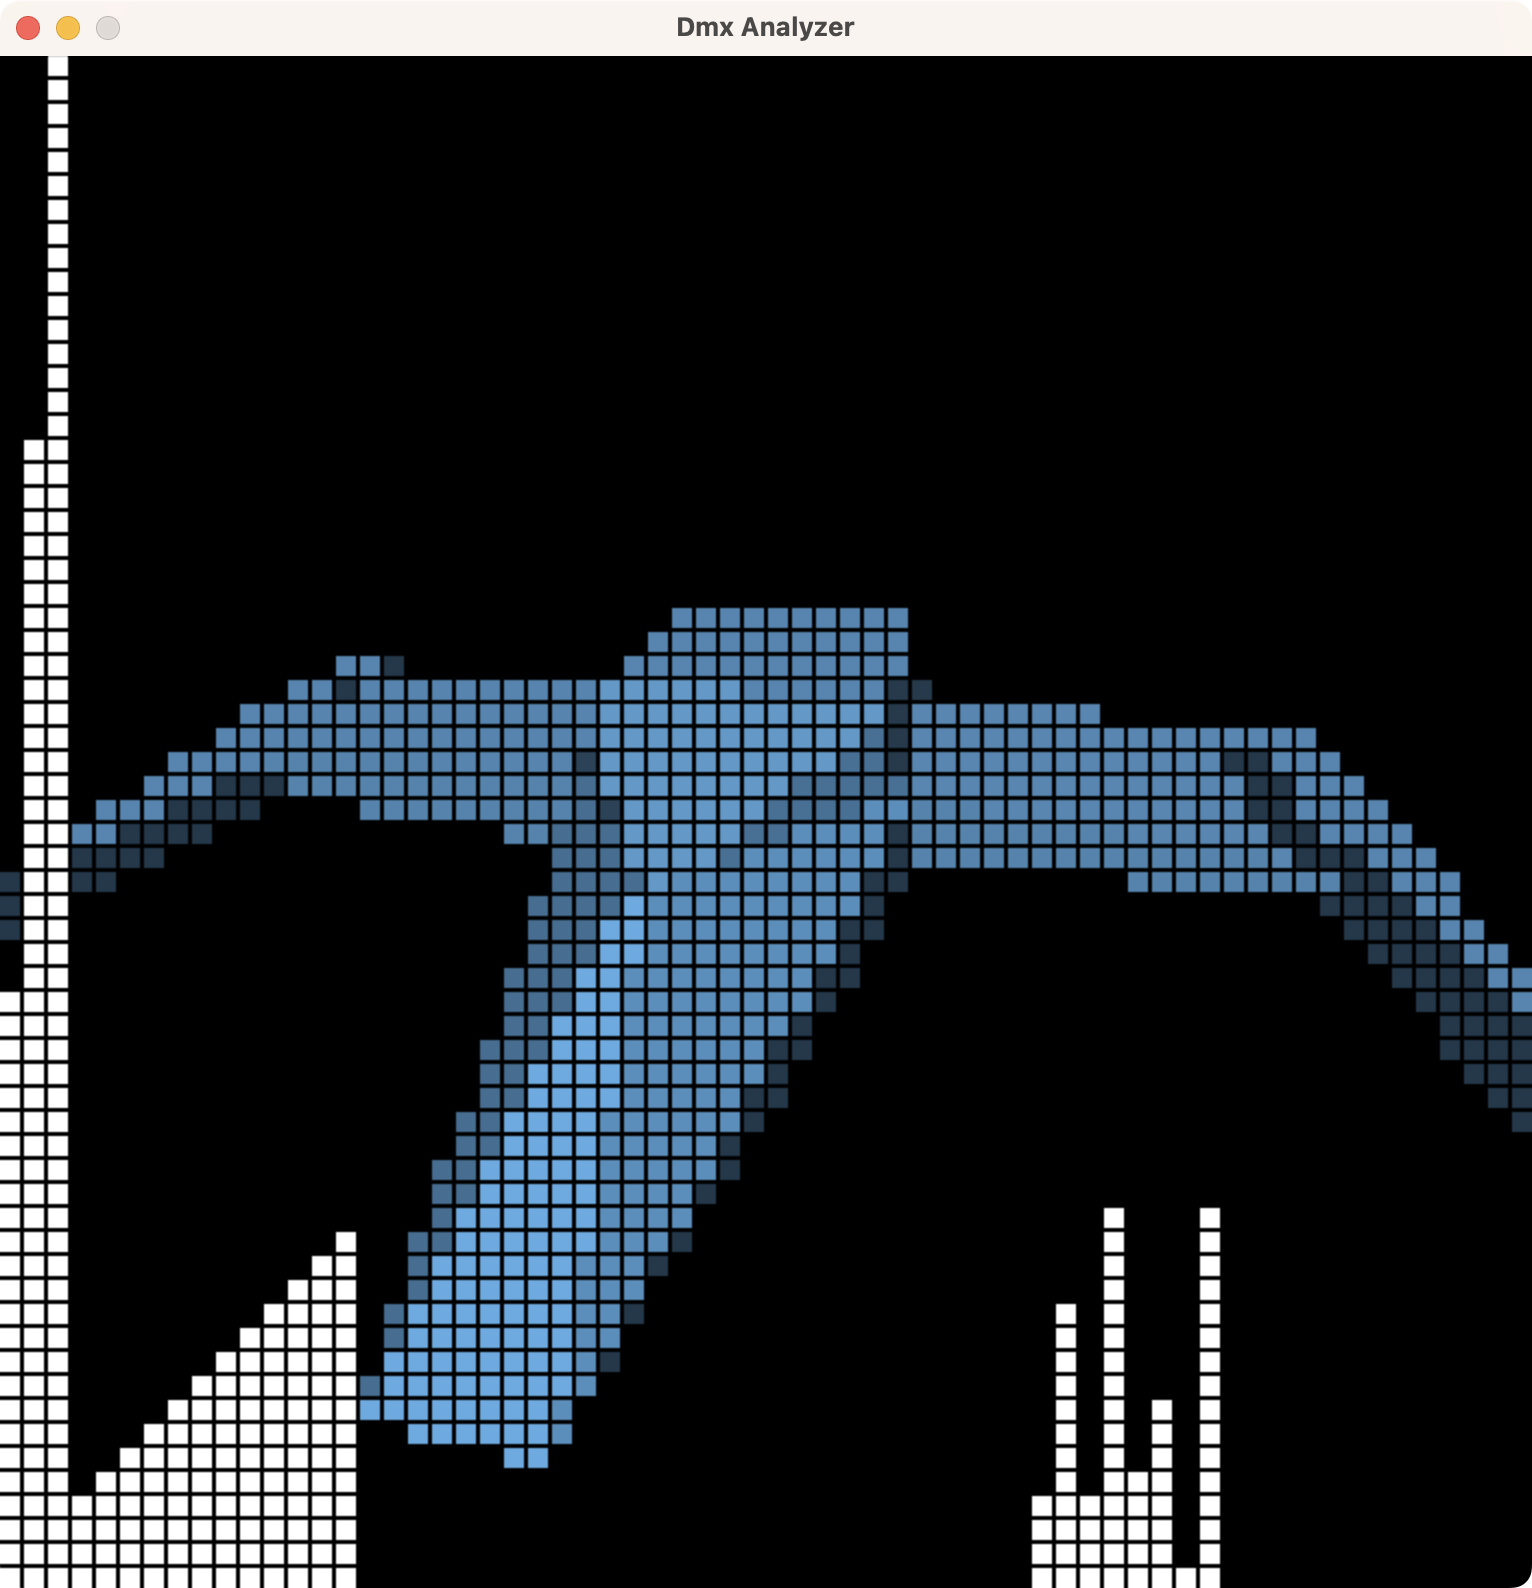
\includegraphics[width=\textwidth/2 - 30pt]{pictures/screenshotRenderCyan}\\
			Farbe: Blau/Cyan
		\end{tabular}
		& 
		\begin{tabular}{c}
			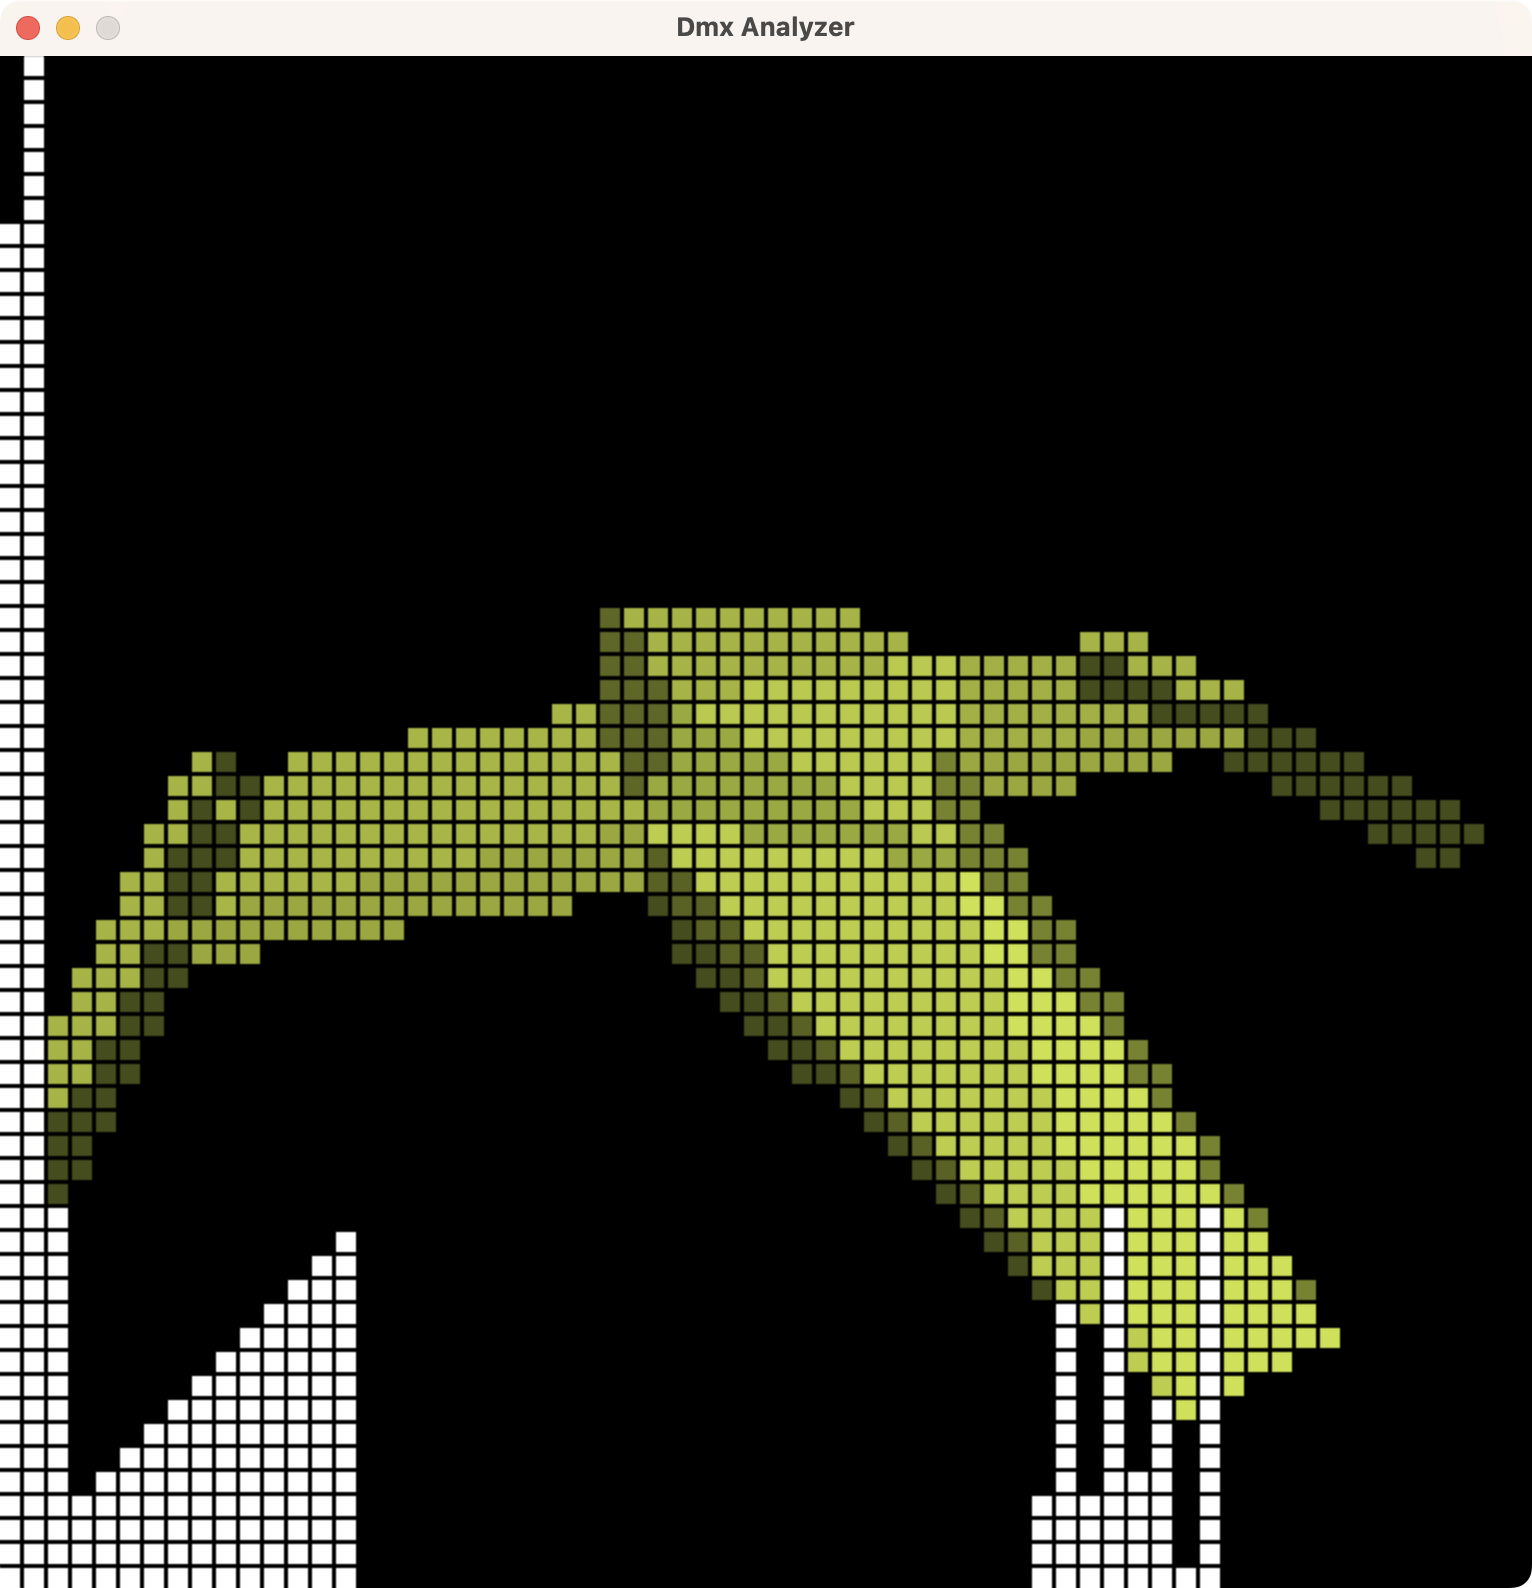
\includegraphics[width=\textwidth/2 - 30pt]{pictures/screenshotRenderYellow}\\
			Farbe: Gelb
		\end{tabular}
	\end{tabular}\\~\\
	Visualisierung von DMX Kanälen mit Beispielanwendung
	\customcite{led-matrix-example}
\end{frame}


\begin{frame}{Danke}
	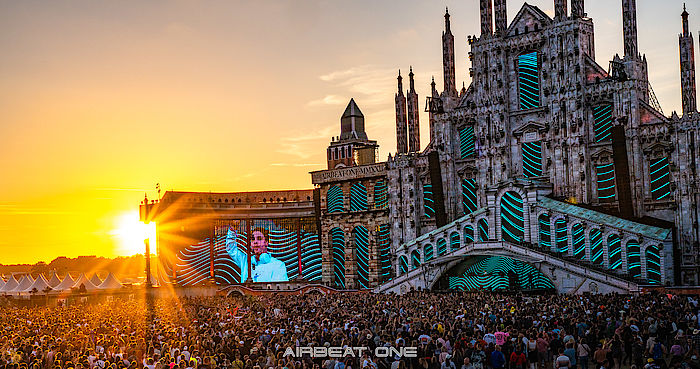
\includegraphics[width=\textwidth - 13pt]{pictures/led-matrix-beispiel}
	\customcite{led_matrix_lightshow}
\end{frame}

\begin{frame}{Quellen}
	\bibliographystyle{unsrtnat} % Use the "unsrtnat" BibTeX style for formatting the Bibliography
	\nocite{cover, banner}
	\scriptsize
	\bibliography{Bibliography}
\end{frame}

\end{document}
